%%%%%%%%%%%%%%%%%%%%%%%%%%%%%%%%%%%%%%%%%
% Sullivan Business Report
% LaTeX Template
% Version 1.0 (May 5, 2022)
%
% This template originates from:
% https://www.LaTeXTemplates.com
%
% Author:
% Vel (vel@latextemplates.com)
%
% License:
% CC BY-NC-SA 4.0 (https://creativecommons.org/licenses/by-nc-sa/4.0/)
%
%%%%%%%%%%%%%%%%%%%%%%%%%%%%%%%%%%%%%%%%%


%----------------------------------------------------------------------------------------
%	CLASS, PACKAGES AND OTHER DOCUMENT CONFIGURATIONS
%----------------------------------------------------------------------------------------

\documentclass[
    a4paper, % Paper size, use either a4paper or letterpaper
	12pt, % Default font size, the template is designed to look good at 12pt so it's best not to change this
	%unnumberedsections, % Uncomment for no section numbering
    ]{CSSullivanBusinessReport}
    
    \addbibresource{sample.bib} % BibLaTeX bibliography file

%----------------------------------------------------------------------------------------
%	REPORT INFORMATION
%----------------------------------------------------------------------------------------

\reporttitle{CPE 233 Hardware Assignment 5} % The report title is to appear on the title page and page headers, do not create manual new lines here as this will carry over to page headers

\reportsubtitle{Branch Condition Generator and Branch Address Generator} % Report subtitle, include new lines if needed

\reportauthors{Report by:\\\smallskip Ethan Vosburg (evosburg@calpoly.edu)} % Report authors/group/department, include new lines if needed

\reportdate{\today} % Report date, include new lines for additional information if needed

\rightheadercontent{
\includegraphics[width=3cm]{creodocs_logo.pdf}} % The content in the right header, you may want to add your own company logo or use your company/department name or leave this command empty for no right header content

%----------------------------------------------------------------------------------------

\begin{document}

%----------------------------------------------------------------------------------------
%	TITLE PAGE
%----------------------------------------------------------------------------------------

\thispagestyle{empty} % Suppress headers and footers on this page

\begin{fullwidth} % Use the whole page width
	\vspace*{-0.075\textheight} % Pull logo into the top margin
	
	\hfill
\includegraphics[width=5cm]{creodocs_logo.pdf} % Company logo

	\vspace{0.15\textheight} % Vertical whitespace

	\parbox{0.9\fulltextwidth}{\fontsize{50pt}{52pt}\selectfont\raggedright\textbf{\reporttitle}\par} % Report title, intentionally at less than full width for nice wrapping. Adjust the width of the \parbox and the font size as needed for your title to look good.
	
	\vspace{0.03\textheight} % Vertical whitespace
	
	{\LARGE\textit{\textbf{\reportsubtitle}}\par} % Subtitle
	
	\vfill % Vertical whitespace
	
	{\Large\reportauthors\par} % Report authors, group or department
	
	\vfill\vfill\vfill % Vertical whitespace
	
	{\large\reportdate\par} % Report date
\end{fullwidth}

\newpage

%----------------------------------------------------------------------------------------
%	DISCLAIMER/COPYRIGHT PAGE
%----------------------------------------------------------------------------------------

% \thispagestyle{empty} % Suppress headers and footers on this page

% \begin{twothirdswidth} % Content in this environment to be at two-thirds of the whole page width
% 	\footnotesize % Reduce font size
	
% 	\subsection*{Disclaimer}

% 	Lorem ipsum dolor sit amet, consectetur adipiscing elit. Praesent porttitor arcu luctus, imperdiet urna iaculis, mattis eros. Pellentesque iaculis odio vel nisl ullamcorper, nec faucibus ipsum molestie. Sed dictum nisl non aliquet porttitor. Etiam vulputate arcu dignissim, finibus sem et, viverra nisl. Aenean luctus congue massa, ut laoreet metus ornare in. Nunc fermentum nisi imperdiet lectus tincidunt vestibulum at ac elit.
	
% 	\subsection*{Copyright}
	
% 	\textcopyright~[Year] [Company] 
	
% 	Copyright notice text\ldots In hac habitasse platea dictumst. Curabitur mattis elit sit amet justo luctus vestibulum. In hac habitasse platea dictumst. Pellentesque lobortis justo enim, a condimentum massa tempor eu. Ut quis nulla a quam pretium eleifend nec eu nisl. Nam cursus porttitor eros, sed luctus ligula convallis quis.
	
% 	\subsection*{Contact}
	
% 	Address Line 1\\
% 	Address Line 2\\
% 	Address Line 3
	
% 	Business Number 123456
	
% 	Contact: name@company.com
	
% 	\vfill % Push the following down to the bottom of the page
	
% 	\subsubsection*{Changelog}
	
% 	\scriptsize % Reduce font size further
	
% 	\begin{tabular}{@{} L{0.05\linewidth} L{0.15\linewidth} L{0.6\linewidth} @{}} % Column widths specified here, change as needed for your content
% 		\toprule
% 		v1.0 & 20XX-02-05 & Lorem ipsum dolor sit amet, consectetur adipiscing elit. Praesent porttitor arcu luctus, imperdiet urna iaculis, mattis eros.\\
% 		v1.1 & 20XX-02-27 & Pellentesque iaculis odio vel nisl ullamcorper, nec faucibus ipsum molestie.\\
% 		v1.2 & 20XX-03-15 & Sed dictum nisl non aliquet porttitor.\\
% 		\bottomrule
% 	\end{tabular}
% \end{twothirdswidth}

% \newpage

%----------------------------------------------------------------------------------------
%	TABLE OF CONTENTS
%----------------------------------------------------------------------------------------
\bigskip
\begin{twothirdswidth} % Content in this environment to be at two-thirds of the whole page width
	\tableofcontents % Output the table of contents, automatically generated from the section commands used in the document
\end{twothirdswidth}

\newpage
%----------------------------------------------------------------------------------------
%	SECTIONS
%----------------------------------------------------------------------------------------
\begin{fullwidth} % Use the whole page width

\section{Project Description} % Top level section

In this project, the branching hardware for the Otter CPU was made. The branch condition generator was created to check the condition given two different source registers. This then resulted in an output of whether or not the values were equal, less than, or less than unsigned. The branch address generator was created to decide where to branch when a branch condition is met. In other words, this unit would modify the program counter given the program counter, j type immediate, b type immediate, i type immediate, and the source register 1. These modules were then formally tested using the SymbiYosys suite and proved to be functional.

\section{Structural Design} % Second level section

\subsection{Branch Address Generator Elaborated Design} % Third level section

\begin{figure}[H]
    \centering
    \captionsetup{style=widetable}
    \makebox[.80\pdfpagewidth]{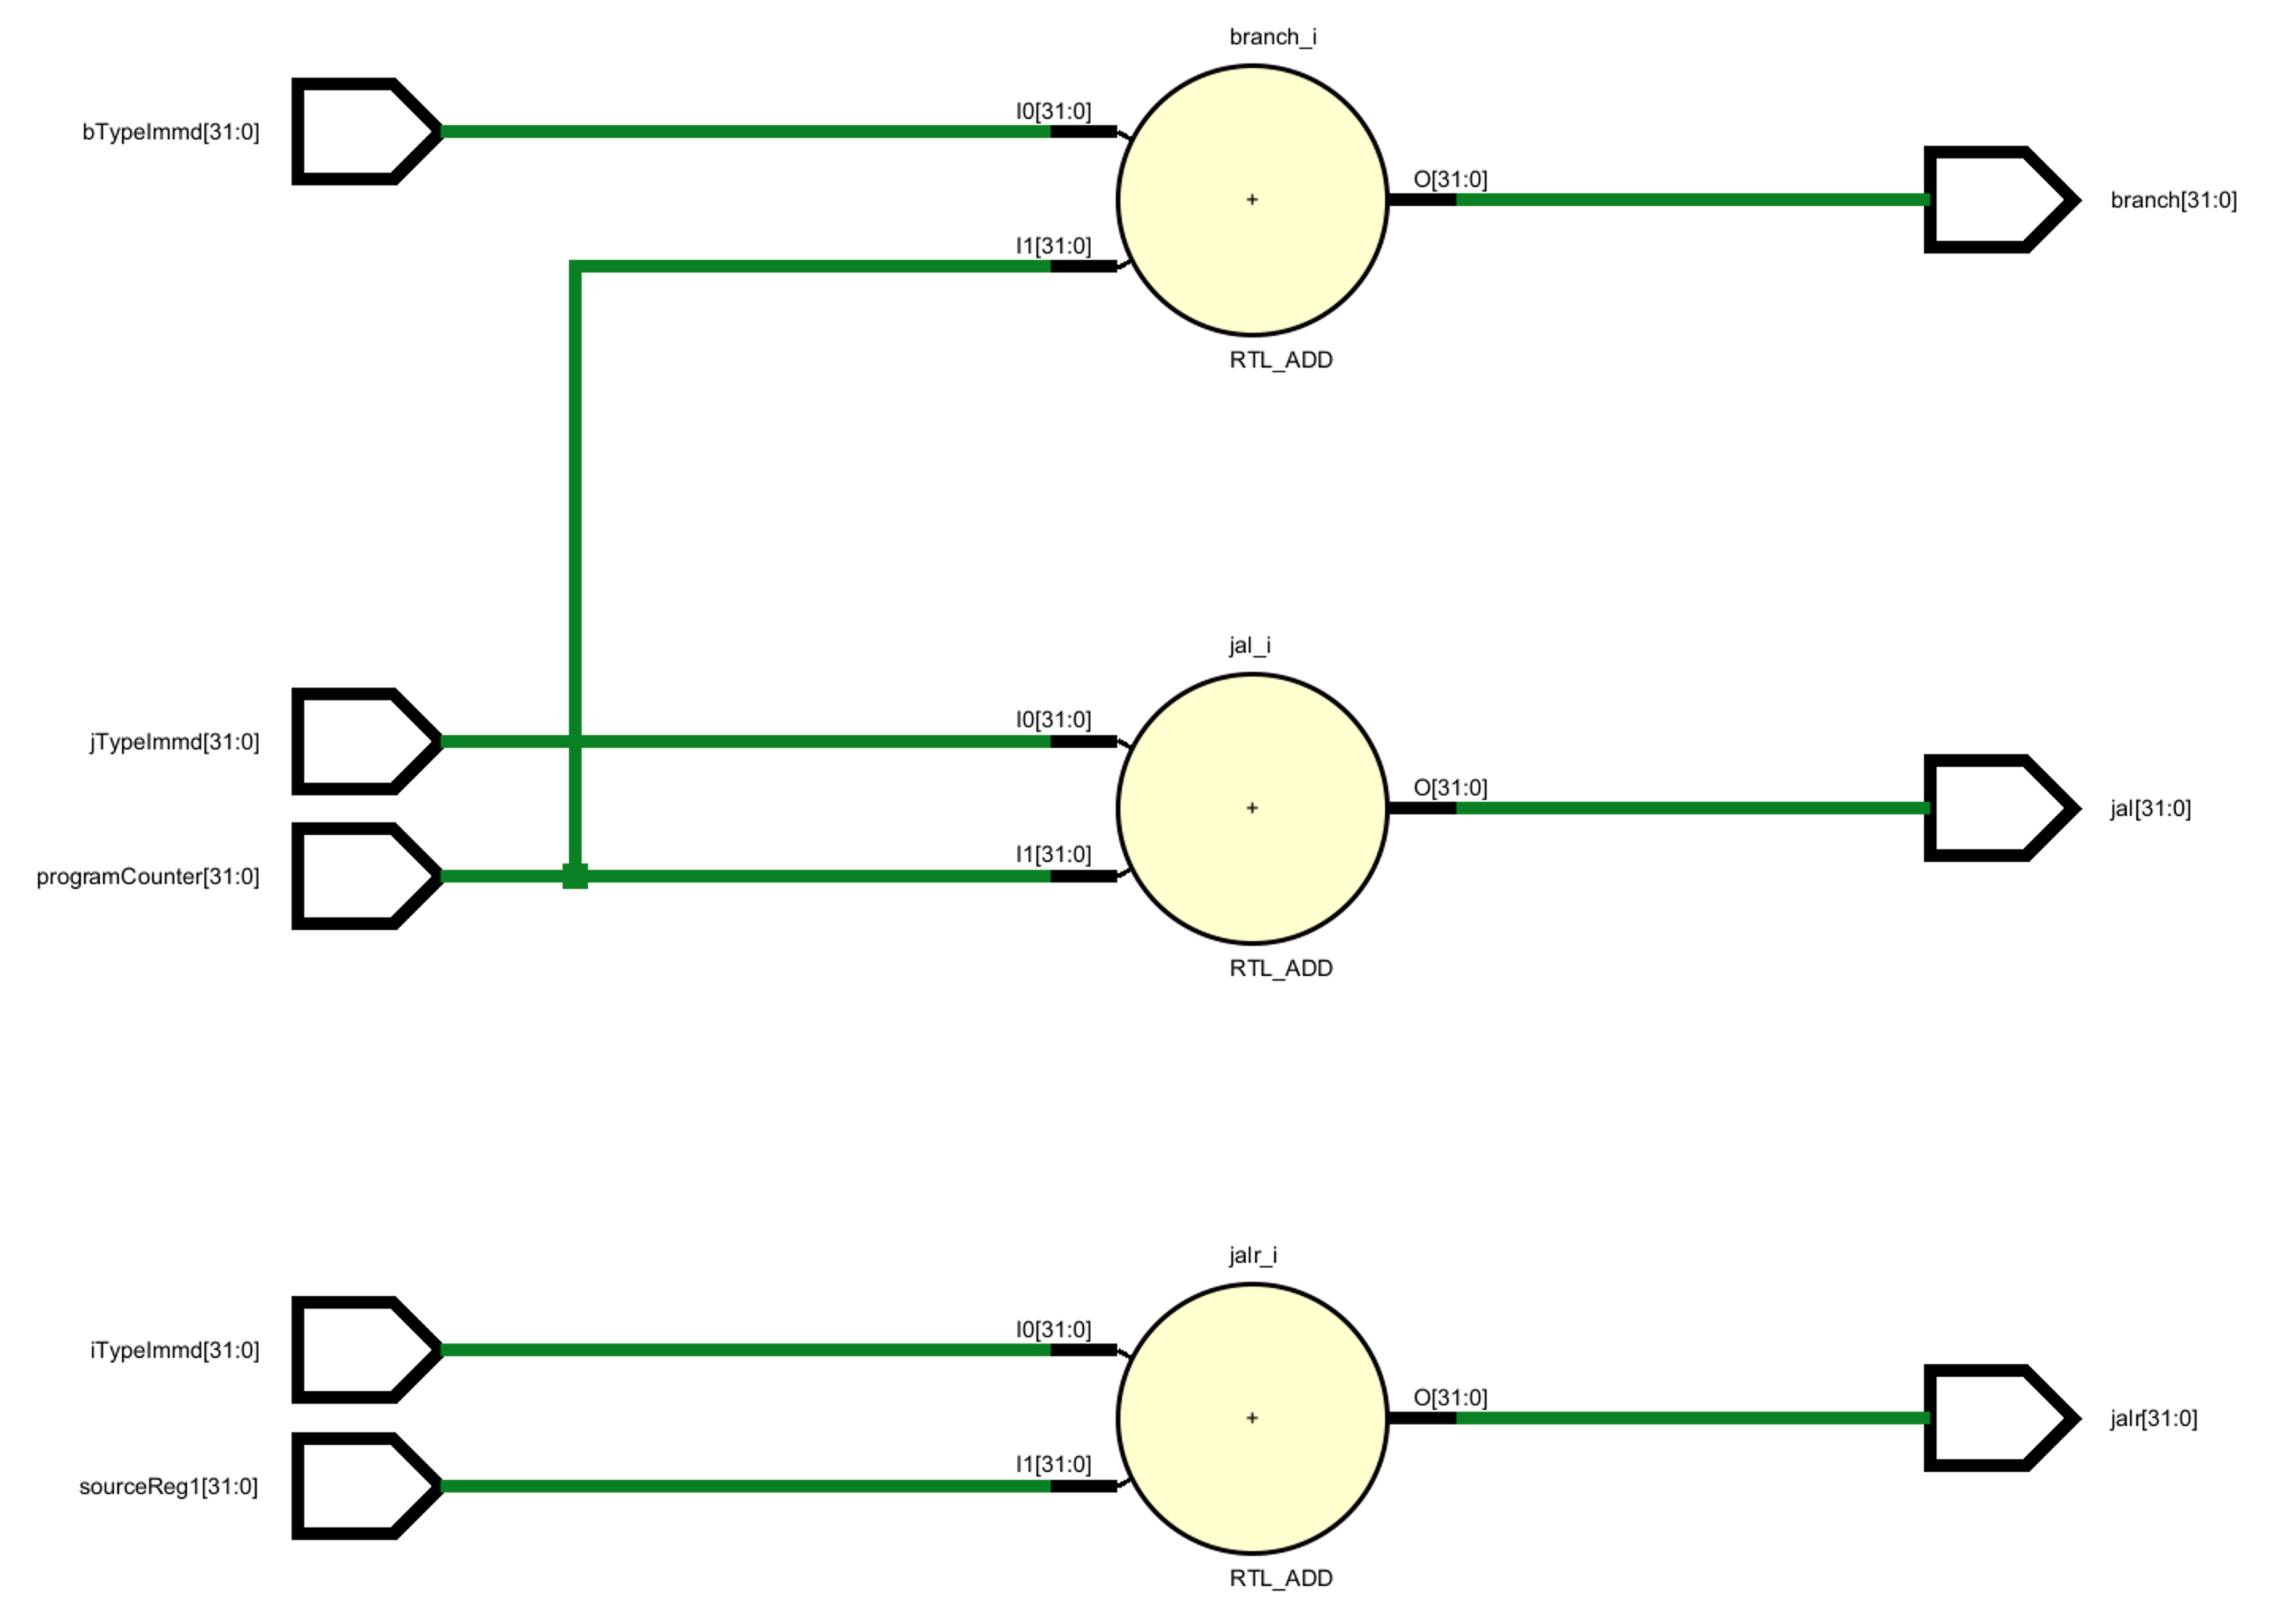
\includegraphics[width=.60\pdfpagewidth]{Figures/Branch Address Generator Elaborated Design.png}}
    \caption{Branch Address Generator Elaborated Design}
    \label{fig:addressDesign}
\end{figure}

The branch address generator combines signals to output a new location for the program counter to jump to. From the elaborated design you can see this process as the different immediate values and registers are combined to get the respective outputs.
\subsection{Branch Condition Generator Elaborated Design} % Third level section
\begin{figure}[H]
    \centering
    \captionsetup{style=widetable}
    \makebox[.80\pdfpagewidth]{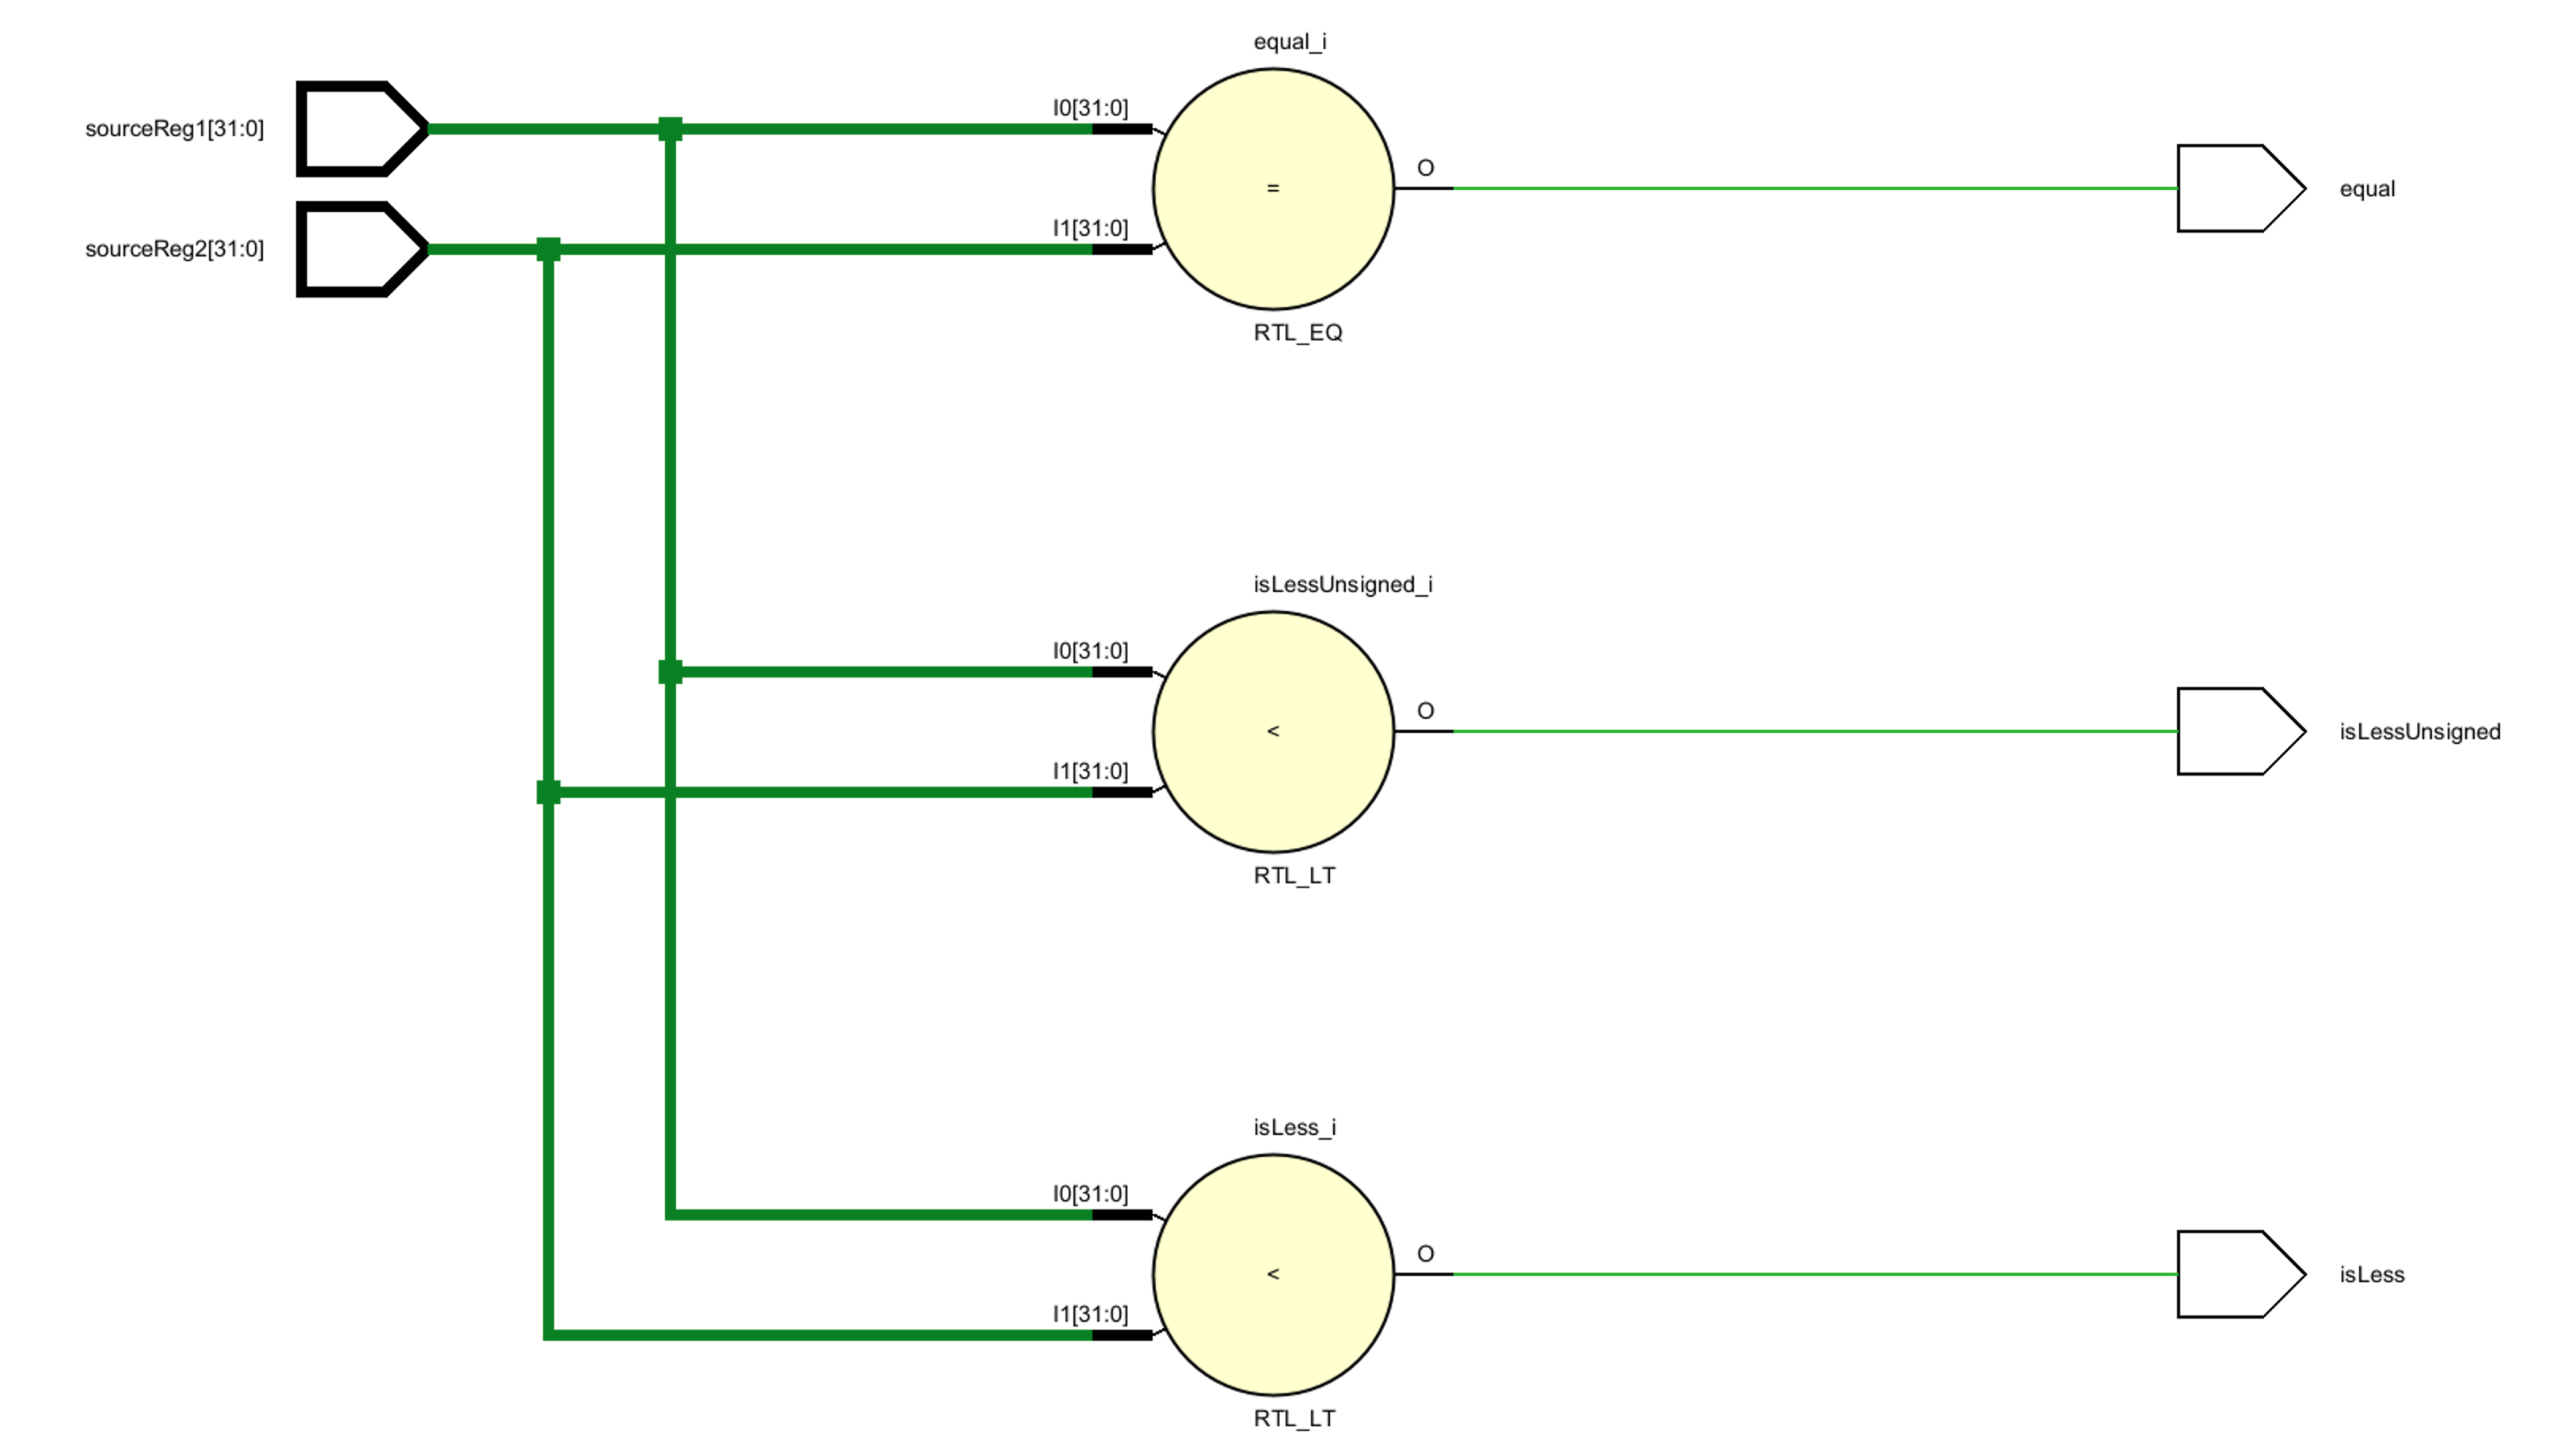
\includegraphics[width=.75\pdfpagewidth]{Figures/Branch Condition Generator Elaborated Design.png}}
    \caption{Branch Condition Generator Elaborated Design}
    \label{fig:conditionDesign}
\end{figure}

The branch condition generator compares the two source registers and then outputs different one-bit values that represent different comparisons. This information can then be used to determine if a branch should be made. 

\subsection{Otter Memory Module Signal Table}
% \begin{adjustbox}{width=\textwidth, center}
\begin{table}[H]
    \rowcolors{2}{gray!25}{white}
    \newcolumntype{M}[1]{>{\centering\arraybackslash}m{#1}}
    \captionsetup{style=widetable}
    % \centering
    \begin{tabular}{|M{1.5in}|M{1.5in}|M{3in}|} \hline 
        Signal Name&  Size (Bits)& Purpose\\ \hline 
        \hline
        MEM\_CLK&  1& This is the clock input for the module\\ \hline 
        MEM\_RDEN1&  1& This is the read enable for the instruction\\ \hline 
        MEM\_RDEN2&  1& This is the read enable for the data\\ \hline 
        MEM\_WE2&  1& This is the write enable\\ \hline 
        MEM\_ADDR1&  14& This is the instruction word memory address that connects to the PC\\ \hline 
        MEM\_ADDR2&  32& This is the data memory address\\ \hline 
        MEM\_DIN2&  32& This is the data that will be saved\\ \hline 
        MEM\_SIZE&  2& This determines the size of the memory that will be saved (0-Byte, 1-Half Word, 2-Word)\\ \hline 
        MEM\_SIGN&  1& This determines whether or not the memory is signed\\ \hline
        IO\_IN& 32&This gets data from the IO of the hardware\\\hline
        \hline
        IO\_WR& 1&This tells the hardware whether data is being read or written\\\hline
        MEM\_DOUT1& 32&This outputs the instruction that is requested by the PC\\\hline
        MEM\_DOUT2& 32&This outputs the data that is requested by the data address\\\hline
    \end{tabular}
    \caption{Otter Memory Module Signal}
    \label{tab:otterMemory}
\end{table}

\section{Synthesis Warnings} % Second level section

\subsection{Branch Address Generator Synthesis Warnings} % Third level section
\begin{figure}[H]
    \captionsetup{style=widetable}
    \makebox[.80\pdfpagewidth]{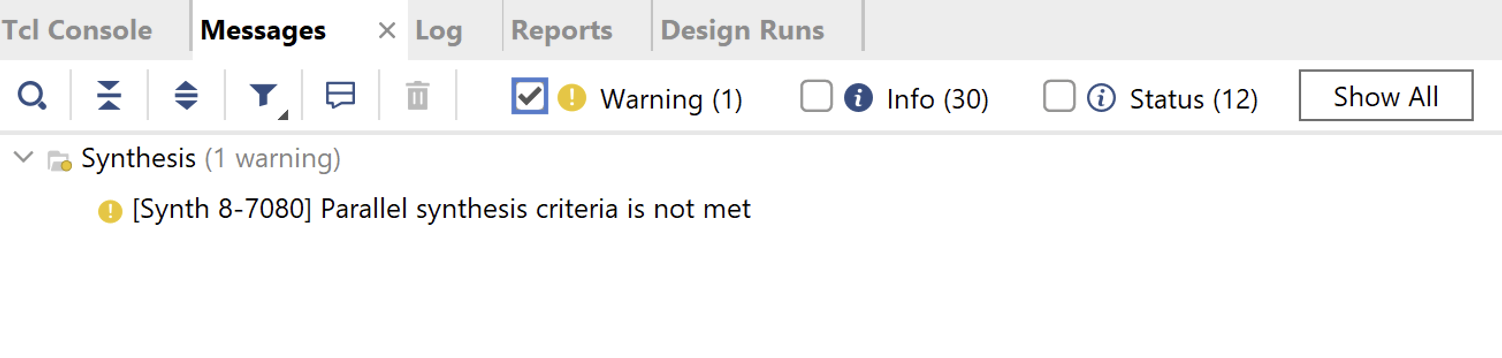
\includegraphics[width=.75\pdfpagewidth]{Figures/Zero Console Warnings.png}}
    \caption{Branch Address Generator Synthesis Warnings}
    \label{fig:addressWarnings}
\end{figure}

\subsection{Branch Condition Generator Synthesis Warnings} % Third level section
\begin{figure}[H]
    \captionsetup{style=widetable}
    \makebox[.80\pdfpagewidth]{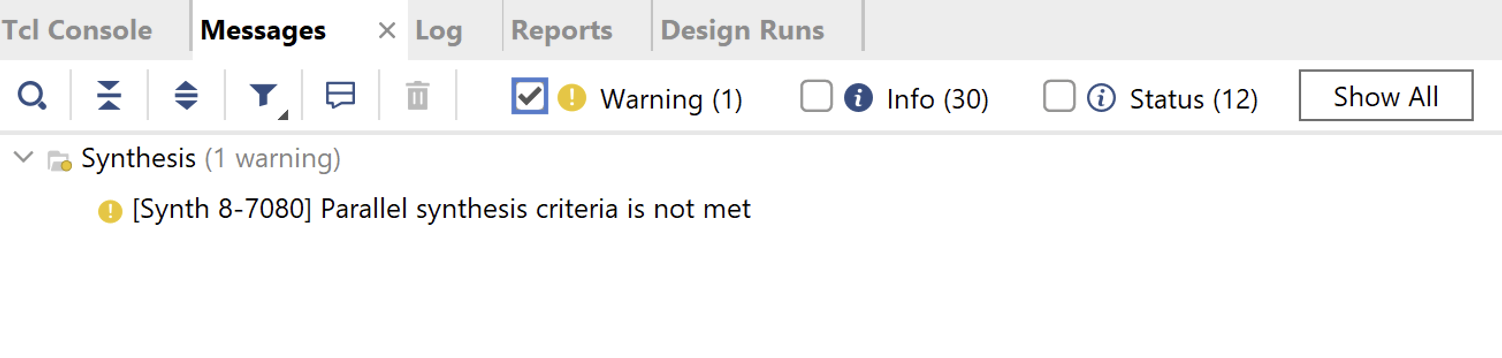
\includegraphics[width=.75\pdfpagewidth]{Figures/Zero Console Warnings.png}}
    \caption{Branch Condition Generator Synthesis Warnings}
    \label{fig:conditionWarnings}
\end{figure}

\section{Verification} % Second level section
In this section, the verification methodology and scope of the verification is explained. A different type of verification was used in this project that allowed for an increased level of confidence when testing the modules.  

\subsection{Verification Methodology and Scope}
Using SymbiYosys, formal verification could be implemented to rigorously test the respective modules. With this testing, the desired function of the code is defined in a separate system verilog file and then that is used to drive an engine to try and break the module that is under test. In this case, two of the three available modes for testing were used Bounded Model Checking(BMC) and Cover. 

Bounded Model Checking is the most basic of the formal testing suit and allows attempts to break the module by using as many different combinations of inputs and outputs as possible. These are not random though, they have mathematical backing to try and break the module that they are testing. 

Cover checking test for coverage of an individual case. This tells the engine to try and figure out how to get to the state that is defined in the code. This is a different process and is more akin to a precise test as you are checking for one thing rather than trying to break a module by any means. 

A general verification process starts with the creation of the module that will be tested. The next step in this process is to generate a formal file that describes the expected behavior of the module that you want to test. It is worth noting that if you want to emphasize test-driven development, this step can be done before the actual programming of the module. The final step is to set up a configuration file that will be used to run the respective tests and set up different criteria. Combined all of these steps allow you to use the SymbiYosys engine to formally verify.

\subsection{Bounded Model Checking} % Third level section

\captionsetup{style=widetable}
For bounded model checking an \verb|assert| statement was used to tell the verification engine to try and break the logic in the test file. An example of this can be seen below in Listing \ref{lst:addressFormalSnipet1}.


\lstinputlisting[label=lst:addressFormalSnipet1, language=Verilog, caption=System Verilog Arithmetic Logic Unit Test Case File, firstline=48, lastline=57]{/Users/ethanvosburg/Documents/git/CPE-233-Otter/HW5-BranchingHardware/BranchingHardware/BranchingHardware.srcs/sources_1/new/BranchAddressGenFormal.sv}

This code will tell the engine what the desired behavior of the module code should be and then will try to break the code by checking different aspects of the inputs and outputs. If a failure is found then a waveform is outputted with the specific conditions needed to break the module.

To see this in action, let's introduce a bug into the \verb|BranchAddressGen.sv| file by changing how the jal line generates its value. In this case, a simple \verb|+ 1| was added to bring the code out of specification.

\lstinputlisting[language=Verilog, caption=Branch Address Generator Introduced Bug, firstline=33, lastline=34]{/Users/ethanvosburg/Documents/git/CPE-233-Otter/HW5-BranchingHardware/BranchingHardware/BranchingHardware.srcs/sources_1/new/BranchAddressGenBug.sv}

Now running this through the verification engine, we get the waveform seen in Figure \ref{fig:addressBug}.

\begin{figure}[H]
    \centering
    \captionsetup{style=widetable}
    \makebox[.80\pdfpagewidth]{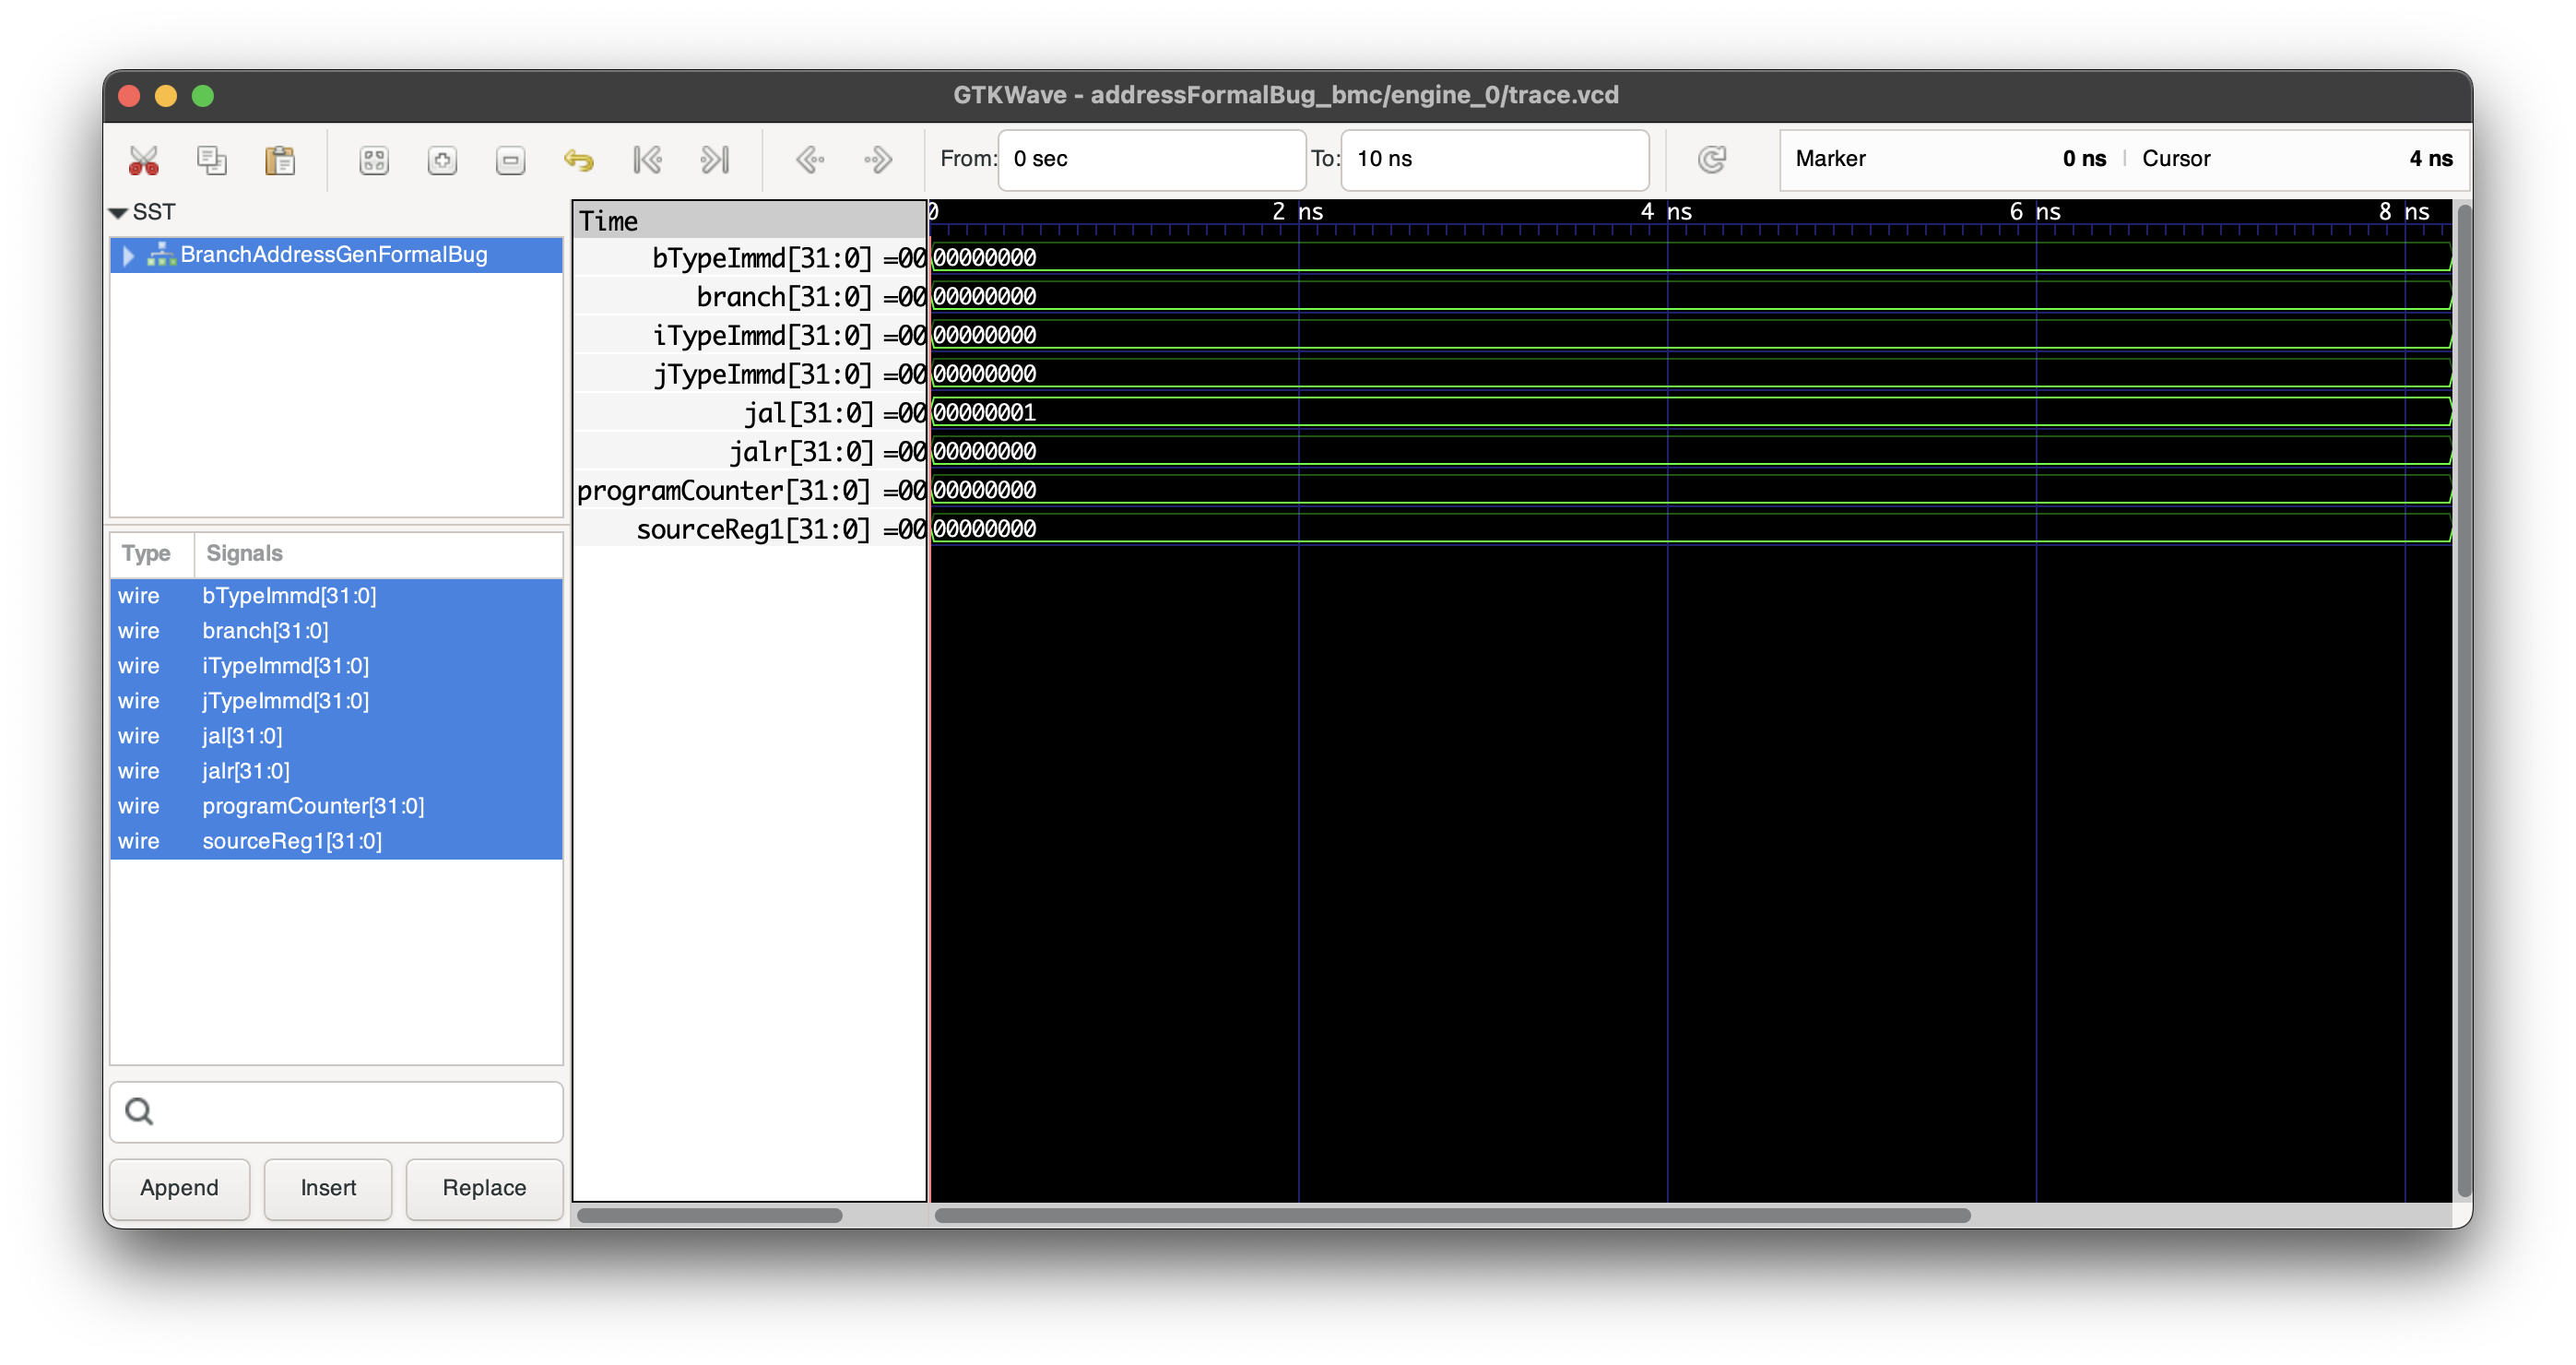
\includegraphics[width=.60\pdfpagewidth]{Figures/BranchAddressBugWaveform.png}}
    \caption{Branch Address Generator Introduced Bug Waverform}
    \label{fig:addressBug}
\end{figure}

Examining Figure \ref{fig:addressBug} we can see that when all zeros are input into the system, we have an output of 1 on the \verb|jal| line which is not what we specified in our testbench when we refer to line 3 of Listing \ref{lst:addressFormalSnipet1}. The engine was able to find this and then error out and show us where the problem is. We can then go to that part of the code and fix that section. The engine was able to break our module and showed that the module that we set up did not work as we described.


\captionsetup{style=widetable}
\subsection{Coverage Verification} % Third level section?
Switching gears, let's look at the cover command in the formal verification suit. This command is used to specify a state that we are looking for and then try to achieve that state in the verification of the code. This is useful when testing to see whether certain conditions are achievable in your code. For example in the snippet below we wish to see if it is possible to reach a state where both the signed and unsigned less-than lines are set. 
\lstinputlisting[label=lst:conditionCoverSnippet, language=Verilog, caption=System Verilog Formal Verification Code for Branch Condition Generator, firstline=56, lastline=57]{/Users/ethanvosburg/Documents/git/CPE-233-Otter/HW5-BranchingHardware/BranchingHardware/BranchingHardware.srcs/sources_1/new/BranchConditionGenFormal.sv}

When running this kind of test, a waveform is generated upon success. When the engine is able to reach the state, it will output what steps it took to get there. The waveform for this specific code is shown below in Figure \ref{fig:coverOut}.

\begin{figure}[H]
    \centering
    \captionsetup{style=widetable}
    \makebox[.80\pdfpagewidth]{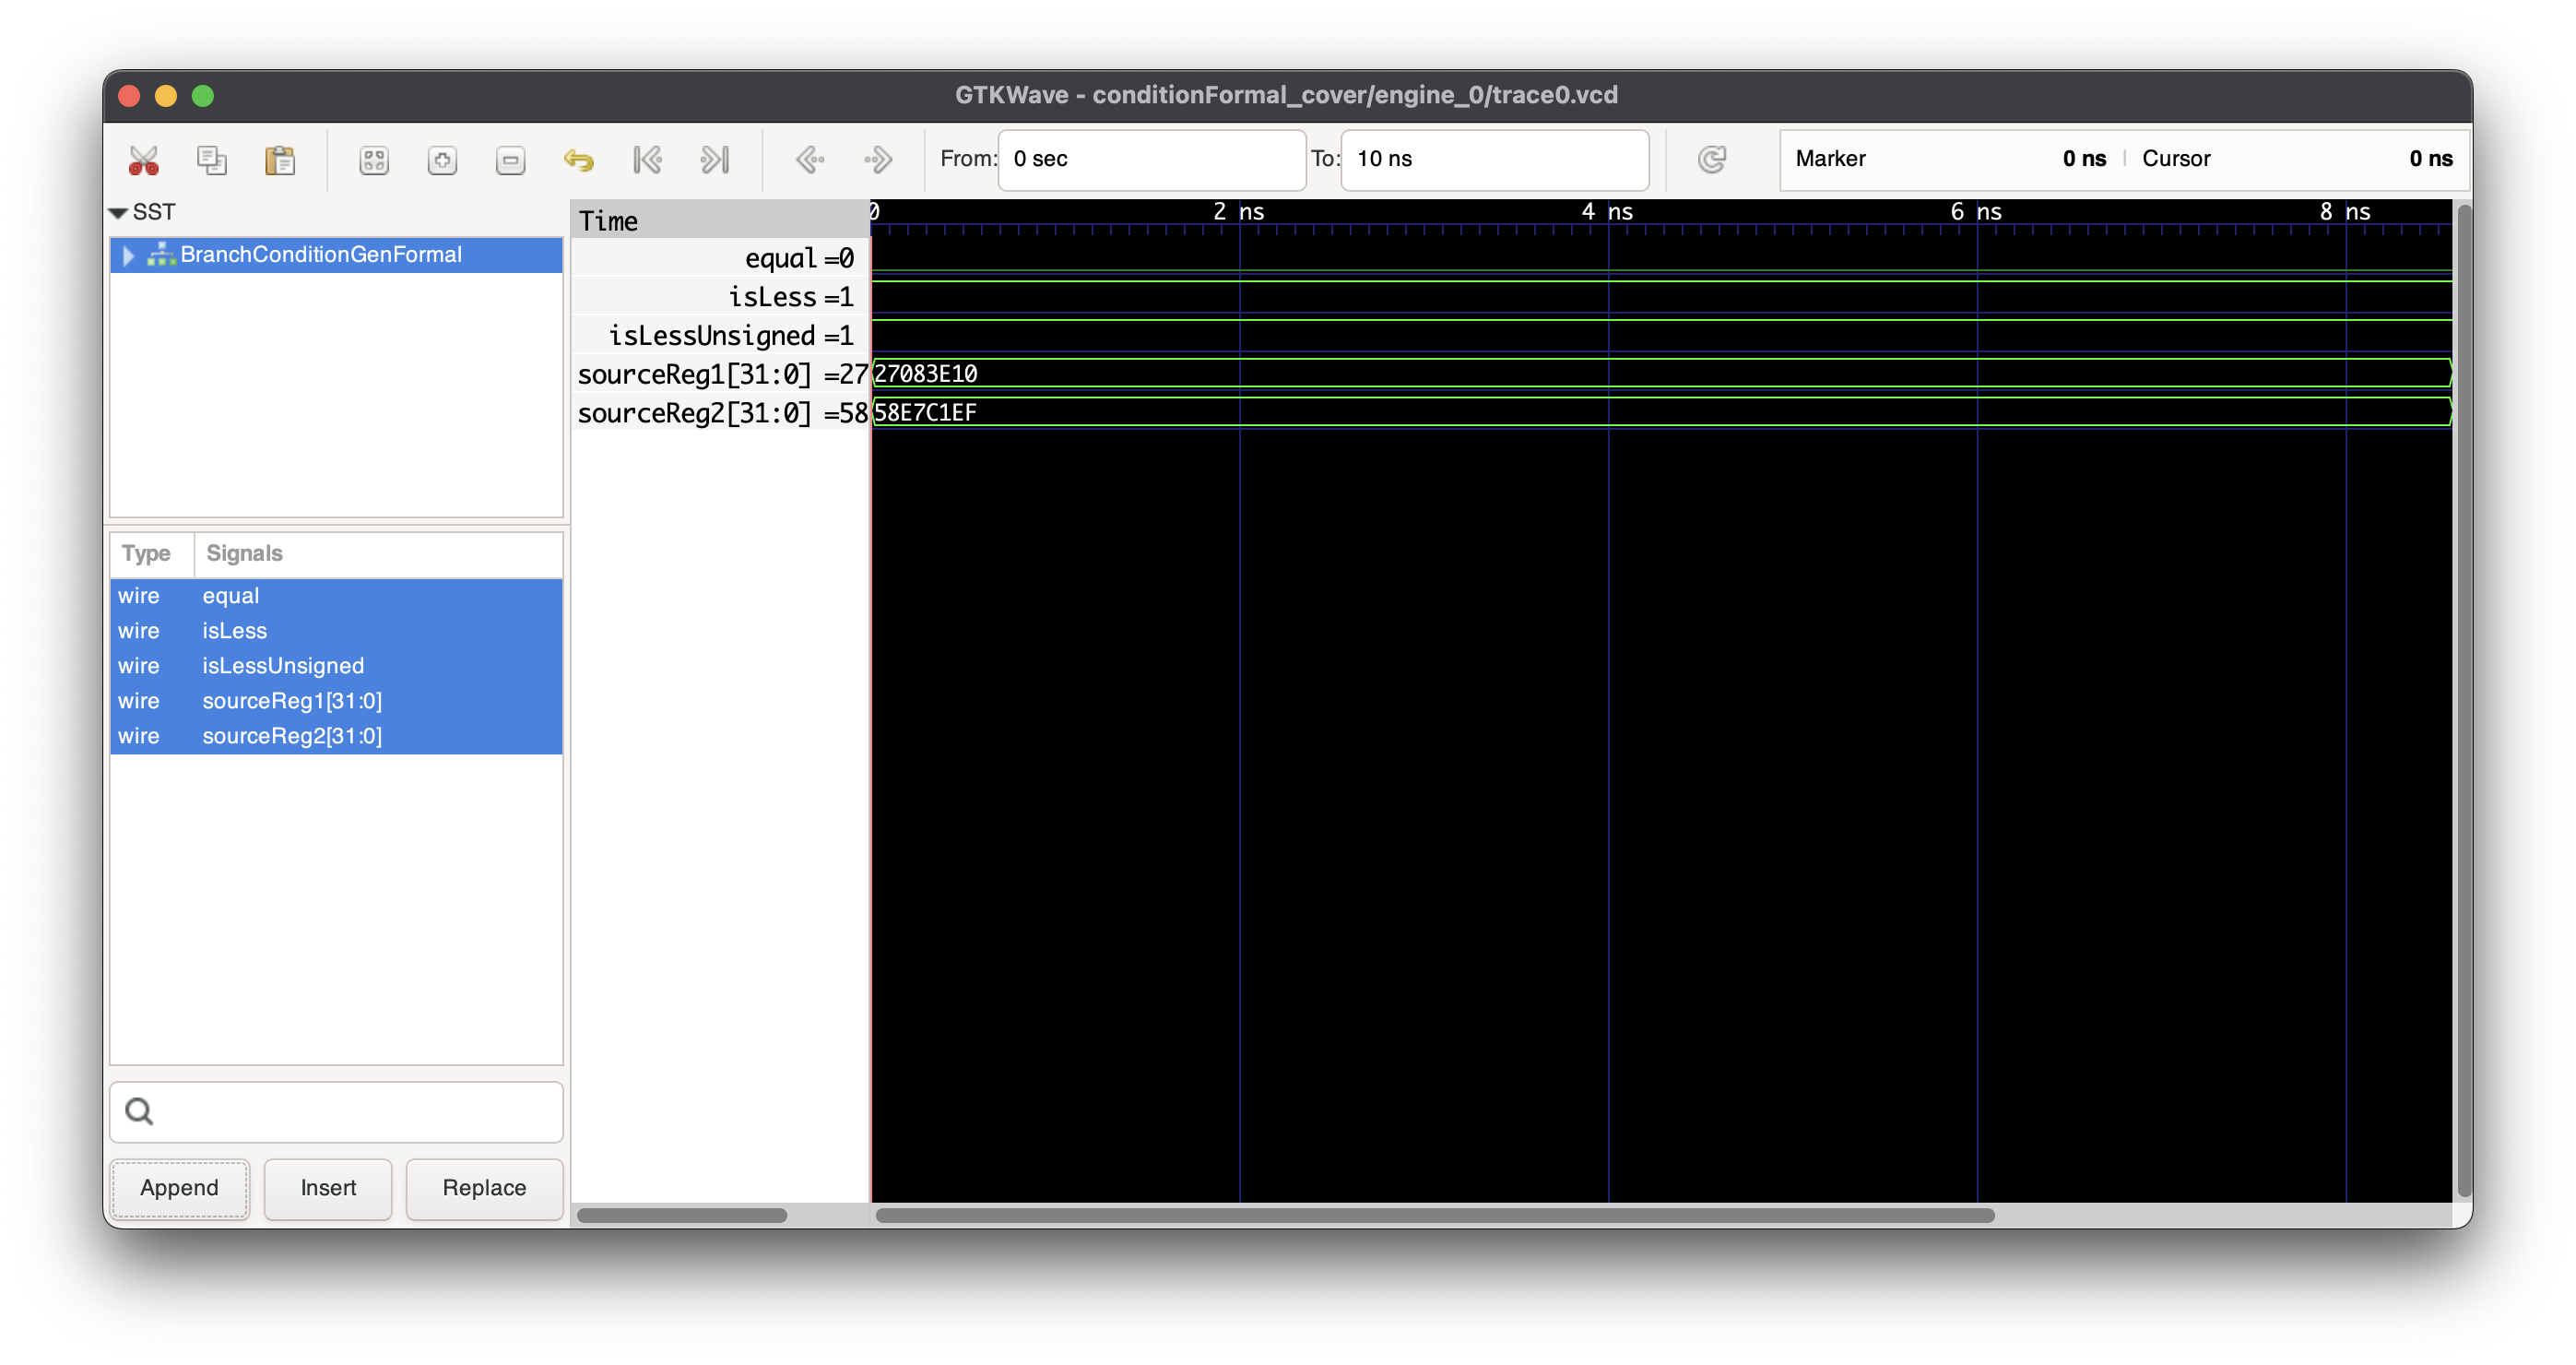
\includegraphics[width=.60\pdfpagewidth]{Figures/ConditionCoverTestWaveform.png}}
    \caption{Branch Condition Generator Cover Test Waveform}
    \label{fig:coverOut}
\end{figure}

This is useful when trying to make sure a critical path can be taken in your module. When designing a complex design, it is possible to introduce unexpected ways to reach a state and this helps with that. You can have the engine try to get to the state and check is that is a valid path. This kind of testing informs you on how to better build your modules.
\newpage
\section{Source Code}
% \captionsetup{style=widetable}
\subsection{Branch Address Generator Source Code} % Third level section

\lstinputlisting[language=Verilog, caption=System Verilog Code for Branch Address Generator]{/Users/ethanvosburg/Documents/git/CPE-233-Otter/HW5-BranchingHardware/BranchingHardware/BranchingHardware.srcs/sources_1/new/BranchAddressGen.sv}
\newpage


\lstinputlisting[language=Verilog, caption=System Verilog Formal Verification Code for Branch Address Generator]{/Users/ethanvosburg/Documents/git/CPE-233-Otter/HW5-BranchingHardware/BranchingHardware/BranchingHardware.srcs/sources_1/new/BranchAddressGenFormal.sv}

\newpage
\lstinputlisting[language=Verilog, caption=SymbiYosys Config File for Branch Address Generator]{/Users/ethanvosburg/Documents/git/CPE-233-Otter/HW5-BranchingHardware/BranchingHardware/BranchingHardware.srcs/sources_1/new/addressFormal.sby}



\subsection{Branch Condition Generator Source Code} % Third level section
\lstinputlisting[language=Verilog, caption=System Verilog Code for Branch Condition Generator]{/Users/ethanvosburg/Documents/git/CPE-233-Otter/HW5-BranchingHardware/BranchingHardware/BranchingHardware.srcs/sources_1/new/BranchConditionGen.sv}

\lstinputlisting[language=Verilog, caption=System Verilog Formal Verification Code for Branch Condition Generator]{/Users/ethanvosburg/Documents/git/CPE-233-Otter/HW5-BranchingHardware/BranchingHardware/BranchingHardware.srcs/sources_1/new/BranchConditionGenFormal.sv}

\newpage
\lstinputlisting[language=Verilog, caption=SymbiYosys Config File for Branch Condition Generator]{/Users/ethanvosburg/Documents/git/CPE-233-Otter/HW5-BranchingHardware/BranchingHardware/BranchingHardware.srcs/sources_1/new/conditionFormal.sby}

% \newpage



\section{Conclusion} % Second level section
\hypersetup{urlcolor=blue} 
Both the branch address generator and branch condition generator hardware were constructed and formally verified. The goal of this hardware was to make decisions on where to branch when a machine code instruction requires branching. Both modules were found to be working as described. Unique to this assignment, formal verification was added and applied to the modules to ensure that they were working properly. Because of this behavioral specification, there was no need for traditional simulation.
All code for this assignment can be found \href{https://github.com/EthanV1920/CPE-233-Otter/tree/main}{here}.


\end{fullwidth}

\end{document}